\chapter{Related Work}

In this section, I want to discuss related work, including work that involves learner corpora (collecting, annotating for special purposes, etc.).

I also want to discuss work that involves automatically evaluating learner responses to tasks, particularly tasks involving a visual reference.

\section{My previous work}
Here I will discuss the work I have previously done in this area, including the papers given in the subsections below.

\subsection{2013}
\cite{king:dickinson:13}

\subsection{2014}
\citet{king:dickinson:14}

\subsection{2016}
\citep{king:dickinson:16}

\subsubsection{Bag-of-dependencies}
Here we could discuss the switch to a bag-of-dependencies approach, the use of tf-idf and the use of vector cosine distance for ranking responses.

\subsubsection{Clustering}
Here we could briefly mention the clustering experiments we did in the 2016 paper. But really, I'd rather not, because I don't intend to repeat them in the dissertation.

\subsection{2018}
\cite{king:dickinson:18}


\section{Other related work}
Here I will discuss work from other researchers that relates to my work. Here are some papers I discussed briefly in my BEA 2018 paper:

\cite{leacock:ea:14}

\cite{kyle2015automatically}

\cite{weigle2013english}

\cite{amaral:meurers:user:07}

\cite{Meurers.Dickinson-17}

\cite{heift:schulze:07}

\cite{somasundaran:ea:15}

\cite{bailey:meurers:08}

\cite{meurers2011evaluating}

\cite{somasundaran:chodorow:14}

\cite{cahill-et-al:14}

\cite{ragheb:dickinson:14a}

\cite{foster2009native}

\cite{cho2013investigating}

\cite{landis1977measurement}

\cite{artstein:massimo:2008}

\cite{tetreault-chodorow:2008:HJCL}

\cite{tetreault:chodorow:08}

% This is a figure in landscape orientation
\begin{sidewaysfigure}
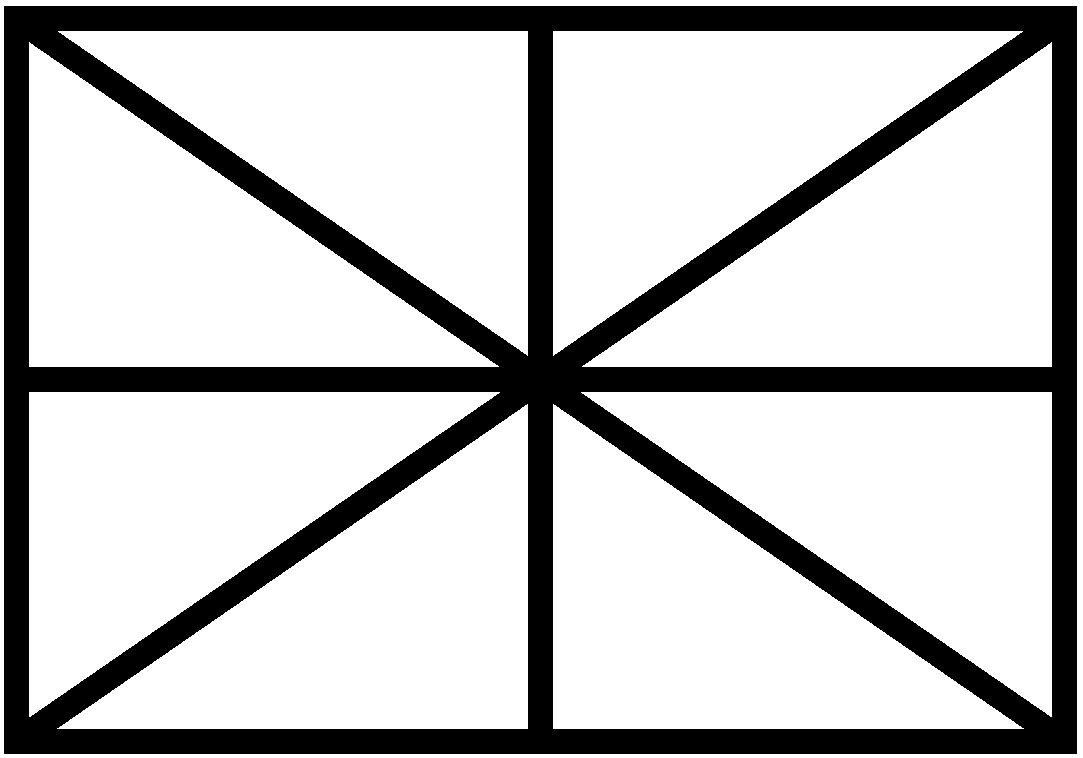
\includegraphics[width=\textwidth]{figures/exampleFigure.png}
\caption{This is another example Figure, rotated to landscape orientation.}
\label{LandscapeFigure}
\end{sidewaysfigure}
